% -----------------------------------------------------------------------------------------------------
% B2. Sources: results/B2_summary.json and the B2 tables of digest.md (start, geometric-mean and end values, d_eff,
% quadratic proxy, monotone fractions, run ends, last-five-pass statistics saga_last5_*, GD end states, minima of
% mu_eff/mu over the kept and over all records, and the criterion 9 n lmin/(16 R^2) under the key crit_9n_lmin_over_16R2);
% GD monotonicity exceptions: keys gd_mu_eff_increasing_steps, gd_mu_eff_increase_max_rel and gd_D_max_after_increase
% (13 of 118 and 56 of 400 GD steps for alpha = 0, kappa = 1e3, 1e4; computed from results/B2.pkl); B2 note
% Rem. B2-P2-outcome, findings.md Sec. 2; order-A shares from B3_summary.json (key shares_orderA); lmin(F''(eta*))/mu
% up to 69.9 over the fifteen B3 problems (B3_summary.json, key mu_local_over_mu). States with mu_eff < mu: only ten
% discarded GD states, for alpha = 2, kappa = 1e2 (iterations 240-249, ||theta_t - eta*||^2 from 6.9e-26 to 9.8e-27,
% mu_eff/mu from 0.993 down to 0.795), computed from results/B2.pkl (the summary stores the minimum under the key
% gd_mu_eff_over_mu_min_all_states).
% -----------------------------------------------------------------------------------------------------
\subsection{Effective curvature along the trajectories (hypothesis B2)}\label{sec:exp-B2}

Are the constants $\muEff(\theta_t)$ and $\LEff(\theta_t)$ of \resref{def:B2-eff}, which make I4 and I2 identities
at the current iterate, much better than $\mu$ and $R^2$, and do they explain the gap (Section~\ref{sec:th-B2})? Along one
SAGA run and one GD run per problem ($\kappa\in\{10^2,10^3,10^4\}$, $\alpha\in\{0,1,2\}$) we record $\muEff/\mu$, $\LEff/R^2$,
the share $\pi_{\min}(t)$ of $\norm{\theta_t-\etastar}^2$ carried by the eigenvector $q_{\min}$ of $F''(\etastar)$ with the
smallest eigenvalue, and the effective number of directions $d_{\rm eff}(t)=1/\sum_k\pi_k(t)^2$ of the error in the
eigenbasis of $F''(\etastar)$, not to be confused with the ridge effective dimension $d_{\rm eff}(\lambda)$ of
Section~\ref{sec:th-B1} (Figure~\ref{fig:B2}).

\begin{figure}[tbp]
  \renewcommand{\thefigure}{B2}% project figure name (see the header of this file)
  \centering
  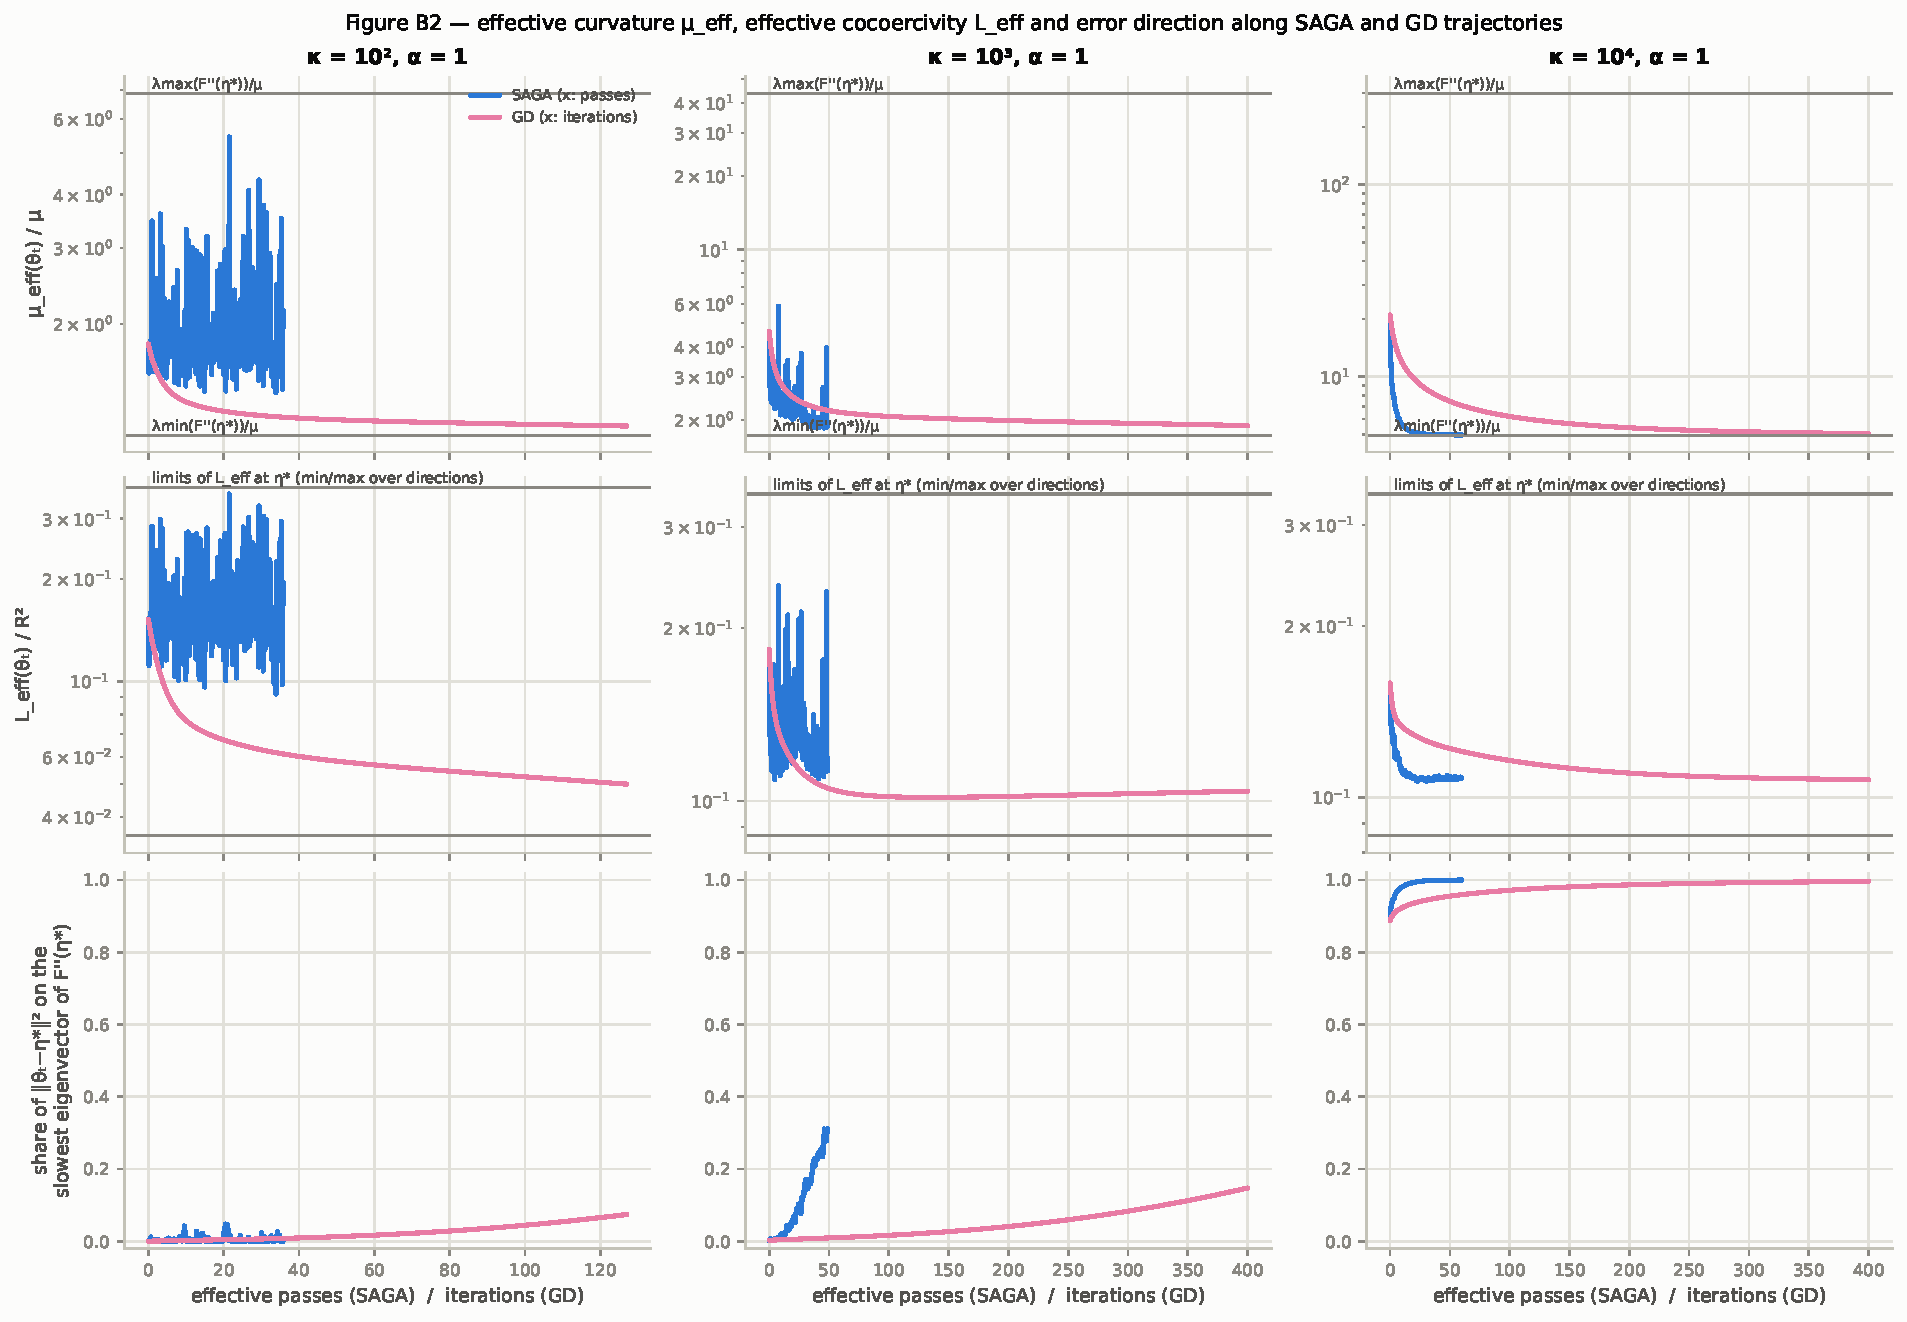
\includegraphics[width=\textwidth]{figB2_effective_curvature}
  \caption{\textbf{Hypothesis B2: effective constants along the trajectories.} $\muEff(\theta_t)/\mu$ (top),
  $\LEff(\theta_t)/R^2$ (middle) and share $\pi_{\min}$ of $\norm{\theta_t-\etastar}^2$ carried by the eigenvector of
  $F''(\etastar)$ with the smallest eigenvalue (bottom), along SAGA (blue, $x$-axis in passes, $\gamma=1/(4R^2)$, at most 60
  passes) and gradient descent (magenta, $x$-axis in iterations, step $1/L_F$, at most 400 iterations), for
  $\kappa\in\{10^2,10^3,10^4\}$ (one column each), $\alpha=1$, $n=1{,}000$, $d=50$, one seed; states with
  $\norm{\theta_t-\etastar}^2<10^{-18}$ are discarded, so that the runs reaching this floor end earlier (SAGA after $36$ and
  $49$ passes for $\kappa=10^2$ and $10^3$, GD after $127$ iterations for $\kappa=10^2$). Horizontal lines:
  $\lmin(F''(\etastar))/\mu$ and $\lmax(F''(\etastar))/\mu$ (top), smallest and largest limits of $\LEff/R^2$ at $\etastar$
  over directions (middle). The configurations $\alpha\in\{0,2\}$ are summarized in Section~\ref{sec:exp-B2}.}
  \label{fig:B2}
\end{figure}

The bound $\muEff\ge\mu$ of \resref{lem:B2-mueff} holds at every retained state (ten discarded GD states below the floor,
at $\alpha=2$, $\kappa=10^2$, give $\muEff/\mu$ between $0.795$ and $0.993$, a rounding artefact), and along SAGA $\muEff/\mu$ starts between
$1.8$ and $50$. The SAGA runs end after 60 passes (last record at pass $59.9$), or after 34 to 49 passes for the five runs
that reach the floor ($\kappa\le10^3$, except $\alpha=2$, $\kappa=10^3$). For $\kappa=10^4$ and $\alpha\in\{0,1\}$ the
error of SAGA concentrates on $q_{\min}$ ($\pi_{\min}=0.998$ and $0.9996$ at the end, $d_{\rm eff}=1.005$ and $1.001$;
from $\theta_0=0$, $\pi_{\min}$ starts at $0.984$ and $0.888$, and for $\alpha=0$ it first drops to $0.938$ at pass
$3.1$), and $\muEff/\mu$ ends within $1\%$ of $\lmin(F''(\etastar))/\mu$ ($9.94$ against $9.86$, $4.97$ against $4.97$);
GD aligns with $q_{\min}$ as well ($\pi_{\min}=1.000$ and $0.996$ after 400 iterations), its $\muEff$ ending at
$\lmin(F''(\etastar))$ and $1.8\%$ above it. For $\kappa=10^2$ the error of SAGA does not concentrate ($\pi_{\min}\le0.05$
over the last five passes, $d_{\rm eff}$ about $18$ and $14$ on average for $\alpha=0,1$) and $\muEff/\mu$ fluctuates
above $\lmin(F''(\etastar))/\mu$ (for $\alpha=1$: geometric mean $1.90$ over the run, between $1.38$ and $3.63$ over the
last five passes, against $1.10$, while GD ends at $1.15$); at $\kappa=10^3$ the alignment is partial ($\alpha=1$:
$\pi_{\min}=0.31$) or absent ($\alpha=0$: $d_{\rm eff}$ about $17$ over the last five passes, while GD is aligned). For
$\alpha=2$ the bottom of the spectrum of $F''(\etastar)$ is nearly degenerate and neither method aligns with $q_{\min}$
(for $\kappa\ge10^3$, GD has moreover not converged after 400 iterations: $\norm{\theta_t-\etastar}^2=5.7\cdot10^{-4}$ and
$202$). Along GD, $\muEff$ is non-increasing at every step up to rounding, as it is exactly on a quadratic by
\resref{prop:B2-gd}: the exceptions, $13$ of $118$ and $56$ of $400$ steps for $\alpha=0$ and $\kappa=10^3$, $10^4$, are
relative increases of at most $7.2\cdot10^{-7}$ and $2.7\cdot10^{-6}$, at states with
$\norm{\theta_t-\etastar}^2\le8.3\cdot10^{-14}$ and $8.1\cdot10^{-13}$. At the end of every SAGA run the quadratic proxy
$\sum_k\lambda_k\pi_k(t)$, with $\lambda_k$ the eigenvalues of $F''(\etastar)$, matches $\muEff$ within $1\%$: near
$\etastar$, $\muEff$ is set by the direction of the error, as \resref{prop:B2-limits} states. The geometric means of
$\LEff/R^2$ along SAGA are $0.19$--$0.38$, $0.11$--$0.16$ and $0.012$--$0.09$ for $\alpha=0,1,2$.

The effective curvature thus exceeds $\mu$ by at least the factor $\lmin(F''(\etastar))/\mu$ near $\etastar$ (up to $9.9$
in these runs, and up to $70$ over the problems of Section~\ref{sec:exp-B3}) and by more far from it, and $\LEff$ is $2.6$
to $86$ times smaller than $R^2$, as hypothesis B2 states. Prediction (P2) of Section~\ref{sec:B2-direction}, that the
error of SAGA stays spread over the directions fed by its noise, holds in the four runs with
$9n\lmin(F''(\etastar))/(16R^2)>1$ ($\kappa=10^2$, and $\kappa=10^3$ with $\alpha=0$) and fails at $\kappa=10^4=10n$ for
$\alpha\in\{0,1\}$, where SAGA aligns with $q_{\min}$ like GD; the three other runs are intermediate (partial alignment at
$\kappa=10^3$, $\alpha=1$; for $\alpha=2$ and $\kappa\ge10^3$, a nearly degenerate bottom spectrum, and neither method
aligns with $q_{\min}$). In terms of $\kappa$ alone, (P2) thus holds only for $\kappa$ at most of the order of $n$, and not in every such
run: $\kappa\approx n$ does not suffice. \resref{rem:B2-P2-outcome} explains the alignment heuristically: when
$n\gamma\lmin(F''(\etastar))$ is small, the iterate moves little during one refresh cycle of the memory, so that the noise
decays with the slowest mode of the mean dynamics instead of at the certified rate (the noise spectrum was not recorded,
so this mechanism is inferred, not measured). For the bound, the one-step factors of \resref{prop:B3-traj} are exactly the
first two steps of order~A of \resref{prop:B3-attribution}: replacing $\mu$ by $\muEff(\theta_{t-1})$ recovers
$0.25$--$0.37$ of the logarithmic gap for $\kappa\ge10^4$ (green curves in Figure~\ref{fig:fig1}), and replacing in
addition $R^2$ by $\LEff(\theta_{t-1})$ in the parameter coefficient recovers $0.59$--$0.96$ (yellow), whereas for
$\kappa\le10^2$ they recover nothing: the bound is then saturated by the memory term, as explained in
\resref{rem:B2-what-explains}. These are a-posteriori statements; the a-priori version, \resref{prop:B3-region}, was not
evaluated along the runs (Section~\ref{sec:th-B3} only computes the rate it gives on a ball around $\etastar$).

% -----------------------------------------------------------------------------------------------------
% B1. Sources: digest.md B1 table, results/B1_summary.json, B1 note (Props. B1-transfer, B1-nofreelunch, B1-diag,
% Rem. B1-memory-bottleneck, predictions (P1)--(P3) and their outcome paragraph), findings.md Sec. 3. Split of the factor
% 3.3-3.8 along order A (memory coefficient 1.95-1.99, I5 1.55-1.70, pathwise remainder 1.10-1.12) and the factor
% 1.10-1.26 invisible in E V_t^P: B1 note, Outcome, and findings.md Sec. 3 (computed from results/B1.pkl).
% -----------------------------------------------------------------------------------------------------
\subsection{SAGA in a fixed quadratic metric (hypothesis B1)}\label{sec:exp-B1}

Does SAGA in the metric of a fixed positive definite $P$, $\theta_t=\theta_{t-1}-\gamma P^{-1}\omega_t$, converge faster,
and which steps of the proof change? By \resref{prop:B1-transfer}, the proof transfers with the relative constants
$(R_P^2,\mu_P)$, which gives \resref{cor:B1-rate}; for logistic regression, no $P$ improves the global condition number:
$\kappaP\ge\kappa$ by \resref{prop:B1-nofreelunch}, restated in Section~\ref{sec:th-B1}. We compare $P=I$, the Jacobi
metric $P_{\rm J}=\diag(\hat\Sigma)+\lambda I$, the statistical metric $\hat\Sigma+\lambda I$ and the Hessian
$F''(\etastar)$, with $\gamma=1/(4R_P^2)$, at $\kappa=10^3$ (Figure~\ref{fig:B1}); here and in the constants below,
$R_P^2$ is the upper bound $\frac14\max_i\norm{x_i}_{P^{-1}}^2+\lambda/\lmin(P)$ of~\eqref{eq:B1-logistic-RP}, exact for
$P=I$ and at most $5.2\%$ above the supremum of \resref{def:B1-kappaP} otherwise. In this order, the exponents per pass of
$\norm{\theta_t-\etastar}_P^2$ (passes 2--20) are $1.00$, $0.94$, $1.11$, $1.11$ for $\alpha=1$ and $0.61$, $0.27$,
$1.26$, $1.24$ for $\alpha=2$. The global constants favour $P=I$ instead: $\kappaP=1000$, $1899$, $5083$, $3623$
($\alpha=1$) and $1000$, $2852$, $3639$, $2089$ ($\alpha=2$) (with the exact supremum, $1000$, $1898$, $5057$, $3611$ and
$1000$, $2841$, $3459$, $2051$), and the certified exponents for $\alpha=1$ are $0.19$, $0.099$, $0.037$, $0.052$. With
the local constant $\lmin(F''(\etastar),P)$ (smallest generalized eigenvalue) in place of $\mu_P$, a heuristic
substitution that \resref{lem:B1-asymptotic} supports only as $\theta\to\etastar$, the relative condition numbers
$R_P^2/\lmin(F''(\etastar),P)$ become $576$, $641$, $166$, $83$ ($\alpha=1$) and $981$, $2433$, $103$, $41$ ($\alpha=2$)
(the condition numbers $\lmax/\lmin$ of $F''(\etastar)$ relative to $P$ are $25$, $26$, $2.8$, $1$ and $50$, $116$, $8.4$,
$1$), and Proposition~\ref{prop:59} so evaluated gives $0.33$, $0.29$, $0.33$, $0.33$ and $0.19$, $0.077$, $0.33$, $0.33$
per pass: the observed ordering, up to the near tie of the dense metrics, which saturate the memory term ($\frac13$ per
pass) while their observed exponents are $3.3$--$3.8$ times larger. In the $P$-geometry the slack moves from cocoercivity
to strong convexity: for $\alpha=1$, $r_{\rm coco}$ rises from $0.13$ to $0.33$--$0.34$ and $r_{\rm sc}$, computed with
the global $\mu_P$, falls from $0.42$ to $0.017$--$0.023$, as prediction (P2) of Section~\ref{sec:B1-predictions} anticipates.

\begin{figure}[tbp]
  \renewcommand{\thefigure}{B1}% project figure name (see the header of this file)
  \centering
  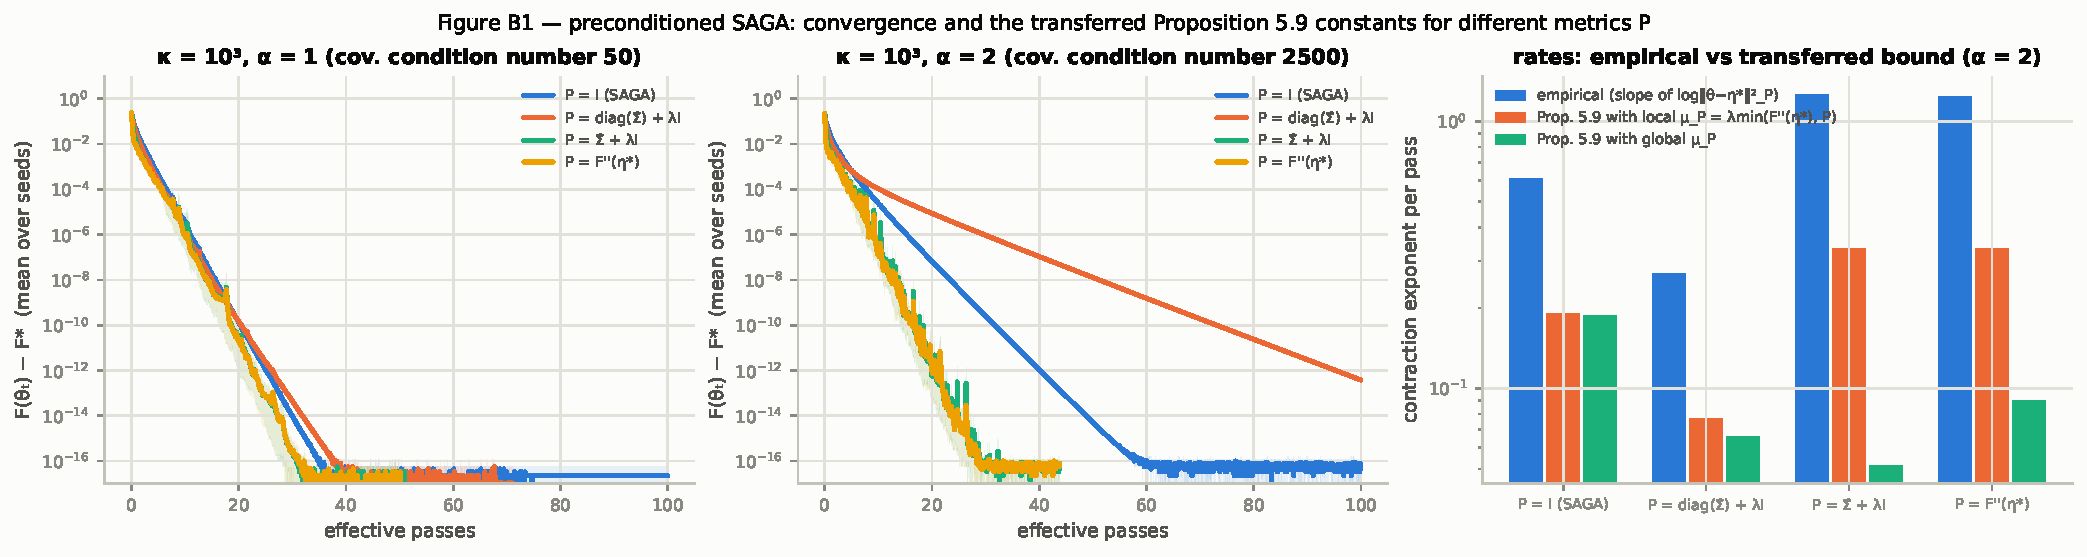
\includegraphics[width=\textwidth]{figB1_preconditioned_saga}
  \caption{\textbf{Hypothesis B1: SAGA in a fixed quadratic metric.} $\theta_t=\theta_{t-1}-\gamma P^{-1}\omega_t$ with
  $\gamma=1/(4R_P^2)$, where $R_P^2=\frac14\max_i\norm{x_i}_{P^{-1}}^2+\lambda/\lmin(P)$ is the upper
  bound~\eqref{eq:B1-logistic-RP} on the transferred smoothness constant, for
  $P\in\{I,\diag(\hat\Sigma)+\lambda I,\hat\Sigma+\lambda I,F''(\etastar)\}$, $\hat\Sigma=\frac1n\sum_ix_ix_i^\top$, on logistic
  regression ($n=1{,}000$, $d=50$, $\kappa=10^3$). Top: $F(\theta_t)-F(\etastar)$ for $\alpha=1$ (left) and $\alpha=2$ (right),
  mean over 5 seeds (band: min--max), up to the end of the shortest run (the runs stop at
  $\norm{\theta_t-\etastar}_P^2\le10^{-26}$). Bottom ($\alpha=2$): contraction exponent per pass of $\norm{\theta_t-\etastar}_P^2$
  (least-squares slope over passes 2--20, mean over seeds) against Proposition~\ref{prop:59} evaluated, heuristically, with
  the local constant $\lmin(F''(\etastar),P)$ (smallest generalized eigenvalue) and with the global constant $\mu_P$.}
  \label{fig:B1}
\end{figure}

The gain of a fixed metric is therefore real but entirely trajectory-dependent: invisible in the global constants, which
cannot improve for logistic regression, it appears in the local ones. Once the curvature is handled by $P$, the bound is
saturated by its memory term, the regime of \resref{rem:B1-memory-bottleneck}, $3.3$ to $3.8$ times below the observed
exponents. Along the measured trajectories (passes 2--20, in the $P$-geometry), this factor splits in three when the
inequalities are undone in order~A of \resref{prop:B3-attribution}, that is, I4, I2, I3, I1, then the min step I5. The memory
coefficient $1-\frac1{3n}$ comes from the textbook weight $\Delta=3\gamma^2$, which absorbs the memory term created by I1
and I3; evaluated exactly by \resref{prop:B3-representation}, with the measured $r_{\rm sq}\approx0.51$--$0.53$ and
$r_{\rm var}\approx1$, it is $1-\frac1n(1-\frac23r_{\rm sq}r_{\rm var})\approx1-\frac{0.65}n$: a factor $1.95$--$1.99$.
The min step I5 charges at the memory rate the parameter part of $V_t^P$, which contracts $7$ to $21$ times faster: a
factor $1.55$--$1.70$. The remaining factor, $1.10$--$1.12$, separates the measured slopes from the exact one-step
contraction. None of this concerns $\E V_t^P$: by the memory recursion~\eqref{eq:B3-EM}, the memory part of $\E V_t^P$
cannot decrease faster than $(1-\frac1n)^t$, so that no bound on $\E V_t^P$ certifies more than about $1$ per pass, $3$
times the local bound, and a factor $1.10$--$1.26$ of the observed exponents is invisible in the expectation that the
analysis controls. The Jacobi metric does not help, and is the slowest for both values of $\alpha$: the features are
randomly rotated, so the diagonal of $\hat\Sigma$ carries little of its anisotropy, and \resref{prop:B1-diag} only places
$P_{\rm J}$ within a factor $\operatorname{cond}(C_{\rm corr})$ of $\hat\Sigma+\lambda I$, in either direction: nothing in
the theory orders $P_{\rm J}$ with respect to $P=I$. The dense metrics cost $O(nd^2)$ per pass, and $P=F''(\etastar)$
requires $\etastar$ (an oracle benchmark).
